%% Generated by Sphinx.
\def\sphinxdocclass{report}
\documentclass[a4paper,12pt,english]{sphinxmanual}
\ifdefined\pdfpxdimen
   \let\sphinxpxdimen\pdfpxdimen\else\newdimen\sphinxpxdimen
\fi \sphinxpxdimen=.75bp\relax

\PassOptionsToPackage{warn}{textcomp}
\usepackage[utf8]{inputenc}
\ifdefined\DeclareUnicodeCharacter
% support both utf8 and utf8x syntaxes
  \ifdefined\DeclareUnicodeCharacterAsOptional
    \def\sphinxDUC#1{\DeclareUnicodeCharacter{"#1}}
  \else
    \let\sphinxDUC\DeclareUnicodeCharacter
  \fi
  \sphinxDUC{00A0}{\nobreakspace}
  \sphinxDUC{2500}{\sphinxunichar{2500}}
  \sphinxDUC{2502}{\sphinxunichar{2502}}
  \sphinxDUC{2514}{\sphinxunichar{2514}}
  \sphinxDUC{251C}{\sphinxunichar{251C}}
  \sphinxDUC{2572}{\textbackslash}
\fi
\usepackage{cmap}
\usepackage[T1]{fontenc}
\usepackage{amsmath,amssymb,amstext}
\usepackage{babel}


\usepackage{amsmath,amsfonts,amssymb,amsthm}

\usepackage{fncychap}
\usepackage[,numfigreset=1,mathnumfig]{sphinx}
\sphinxsetup{hmargin={0.7in,0.7in}, vmargin={1in,1in},         verbatimwithframe=true,         TitleColor={rgb}{0.443,0.160,0.282},         HeaderFamily=\rmfamily\bfseries,         InnerLinkColor={rgb}{0.443,0.160,0.282},         OuterLinkColor={rgb}{0.443,0.160,0.282}}
\fvset{fontsize=\small}
\usepackage{geometry}


% Include hyperref last.
\usepackage{hyperref}
% Fix anchor placement for figures with captions.
\usepackage{hypcap}% it must be loaded after hyperref.
% Set up styles of URL: it should be placed after hyperref.
\urlstyle{same}
\addto\captionsenglish{\renewcommand{\contentsname}{Contents:}}

\usepackage{sphinxmessages}
\setcounter{tocdepth}{1}


        %%%%%%%%%%%%%%%%%%%% DD Settings %%%%%%%%%%%%%%%%%%
        %%%add number to subsubsection 2=subsection, 3=subsubsection
        %%% below subsubsection is not good idea.
        \setcounter{secnumdepth}{3}
        %
        %%%% Table of content upto 2=subsection, 3=subsubsection
        \setcounter{tocdepth}{2}

        \usepackage{amsmath,amsfonts,amssymb,amsthm}
        \usepackage{graphicx}
        \usepackage[export]{adjustbox}

        %%% reduce spaces for Table of contents, figures and tables
        %%% it is used "\addtocontents{toc}{\vskip -1.2cm}" etc. in the document
        \usepackage[notlot,nottoc,notlof]{}

        \usepackage{color}
        \usepackage{transparent}
        \usepackage{eso-pic}
        \usepackage{lipsum}

        \usepackage{footnotebackref} %%link at the footnote to go to the place of footnote in the text

        %% spacing between line
        \usepackage{setspace}
        %%%%\onehalfspacing
        %%%%\doublespacing
        \singlespacing


        %%%%%%%%%%% datetime
        \usepackage{datetime}

        \newdateformat{MonthYearFormat}{%
            \monthname[\THEMONTH], \THEYEAR}


        %% RO, LE will not work for 'oneside' layout.
        %% Change oneside to twoside in document class
        \usepackage{fancyhdr}
        \pagestyle{fancy}
        \fancyhf{}

        %%% Alternating Header for oneside
        \fancyhead[L]{\ifthenelse{\isodd{\value{page}}}{ \small \nouppercase{\leftmark} }{}}
        \fancyhead[R]{\ifthenelse{\isodd{\value{page}}}{}{ \small \nouppercase{\rightmark} }}

        %%% Alternating Header for two side
        %\fancyhead[RO]{\small \nouppercase{\rightmark}}
        %\fancyhead[LE]{\small \nouppercase{\leftmark}}

        %% for oneside: change footer at right side. If you want to use Left and right then use same as header defined above.
        \fancyfoot[R]{\ifthenelse{\isodd{\value{page}}}{{\tiny Dirk Leese} }{\href{http://www.logipad.aerol}{\tiny visit Logipad ebsite }}}

        %%% Alternating Footer for two side
        %\fancyfoot[RO, RE]{\scriptsize Dirk Leese (dirk.leese@dextradata.com)}

        %%% page number
        \fancyfoot[CO, CE]{\thepage}

        \renewcommand{\headrulewidth}{0.5pt}
        \renewcommand{\footrulewidth}{0.5pt}

        \RequirePackage{tocbibind} %%% comment this to remove page number for following
        \addto\captionsenglish{\renewcommand{\contentsname}{Table of contents}}
        \addto\captionsenglish{\renewcommand{\listfigurename}{List of figures}}
        \addto\captionsenglish{\renewcommand{\listtablename}{List of tables}}
        % \addto\captionsenglish{\renewcommand{\chaptername}{Chapter}}


        %%reduce spacing for itemize
        \usepackage{enumitem}
        \setlist{nosep}

        %%%%%%%%%%% Quote Styles at the top of chapter
        \usepackage{epigraph}
        \setlength{\epigraphwidth}{0.8\columnwidth}
        \newcommand{\chapterquote}[2]{\epigraphhead[60]{\epigraph{\textit{#1}}{\textbf {\textit{--#2}}}}}
        %%%%%%%%%%% Quote for all places except Chapter
        \newcommand{\sectionquote}[2]{{\quote{\textit{``#1''}}{\textbf {\textit{--#2}}}}}
    

\title{eForms}
\date{May 11, 2020}
\release{1.0.0}
\author{Dirk Leese}
\newcommand{\sphinxlogo}{\sphinxincludegraphics{logipad-aero-logo-black.png}\par}
\renewcommand{\releasename}{ }
\makeindex
\begin{document}

\pagestyle{empty}

        \pagenumbering{Roman} %%% to avoid page 1 conflict with actual page 1

        \begin{titlepage}
            \centering
            \vspace*{0mm} %%% * is used to give space from top
            \begin{figure}[!h]
                \vspace*{-20mm}
                
\includegraphics[right]{/Users/dl/develop/lp-docs/eforms/source/_images/DD-logo.png}
            \end{figure}
            \vspace{30mm} %%% * is used to give space from top
            \begin{figure}[!h]
                \centering
                
\includegraphics[scale=1.0]{/Users/dl/develop/lp-docs/eforms/source/_images/logipad-aero-logo-black.png}
            \end{figure}

            \vspace{10mm} 
            \textbf{\Huge {eForms User Guide}}

            \vspace{30mm}
            \Large \textbf{{Dirk Leese}}

            \small Created on : \today

            \vspace*{0mm}
            \small  Last updated : \MonthYearFormat\today
            
            \vspace{70mm}
            \begin{figure}[!h]
                \hspace*{-20mm}
                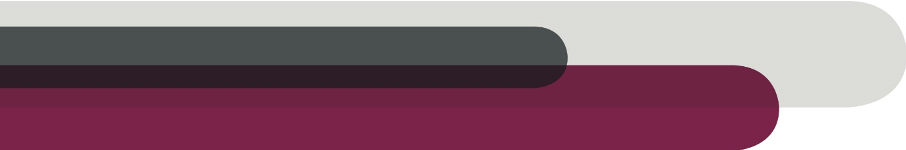
\includegraphics[scale=1.0,left]{/Users/dl/develop/lp-docs/eforms/source/_images/DD-stripes.png}
            \end{figure}
            %% \vfill adds at the bottom
            \vfill
            \small \textit{More information are available at }{\href{http://www.logipad.aero}{Logpad}}
        \end{titlepage}

        \clearpage
        \pagenumbering{roman}
        \tableofcontents
        \listoffigures
        \listoftables
        \clearpage
        \pagenumbering{arabic}

        
\pagestyle{plain}
 
\pagestyle{normal}
\phantomsection\label{\detokenize{index::doc}}



\chapter{eForms}
\label{\detokenize{eForms:eforms}}\label{\detokenize{eForms::doc}}
Electronic forms have become more and more important as digitization and automatic data processing has progressed. eForms are not limited to simple text input or selection fields.

eForms are not limited to simple text input or selection fields. Data input can be automated using the integrated QR code scanner, for example. No matter whether they record flight\sphinxhyphen{}relevant data or performance evaluations of service personnel. You have the option of evaluating the data via an individual dashboard or in Power BI. All entered data is stored on the device for offline use. Once a Wi\sphinxhyphen{}Fi or mobile data connection is established, completed eForm inputs can be sent to the backend system. Even workflows and notifications can be triggered to inform the relevant users/roles when, when eForms have been stored or have arrived on the server. Documents and photos can also be attached and forwarded via an appropriate eForm.

\begin{figure}[htbp]
\centering
\capstart

\noindent\sphinxincludegraphics[scale=0.5]{{Logipad-eForms-web}.png}
\caption{The eForm process}\label{\detokenize{eForms:id1}}\end{figure}


\section{eForm Generator}
\label{\detokenize{eForms:eform-generator}}
The Logipad eForms Module allows you to create your own electronic forms with our intuitive eForm drag and drop editor or use existing templates. The video shows how easy and intuitive it is to create eForms yourself with Logipad.


\chapter{About Logipad}
\label{\detokenize{about:about-logipad}}\label{\detokenize{about::doc}}
Initially, Logipad was developed upon a request of a customer: In 2002, the airline LTU commissioned us to develop an Electronic Flight Bag solution. Since then, Logipad has been further developed and improved as a valuabe solution for the aircraft industry.
In 2002, T\&A Systeme, later known as Modern.Work, has been providing airlines with the inhouse\sphinxhyphen{}developed Electronic Flight Bag solution. In 2017, Modern.Work merged with DextraData, an IT consulting company and independent software vendor.
DextraData, located in Germany with offices in Essen, Hamburg and Munich, offers comprehensive expertise in IT services and EFB. Our aim is to implement and develop IT solutions according to customer requirements.


\chapter{Indices and tables}
\label{\detokenize{index:indices-and-tables}}\begin{itemize}
\item {} 
\DUrole{xref,std,std-ref}{genindex}

\item {} 
\DUrole{xref,std,std-ref}{modindex}

\item {} 
\DUrole{xref,std,std-ref}{search}

\end{itemize}



\renewcommand{\indexname}{Index}
\printindex
\end{document}